
\subsection*{Trabajos Futuros}
\noindent
Como hemos indicado anteriormente, existe una variedad importante de dispositivos electr�nicos en los que se puede usar un l�piz. Sin embargo, todav�a no hay una aplicaci�n sobresaliente para tales dispositivos. El usuario ve al stylus como un mouse sofisticado.

Vemos en la matem�tica una aplicaci�n que puede cambiar el estado actual. No s�lo escribir en matem�tica sino tambi�n trabajar con expresiones, ya que actualmente existen poderosos sistemas de c�lculo simb�lico, como Maple \cite{Maple}.

Una obvia motivaci�n es el hecho de que escribir matem�tica en una computadora es problem�tico. Por ejemplo, la expresi�n:
\begin{figure}[!htbp]
    \centering
    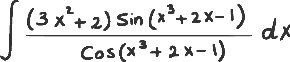
\includegraphics{imagen/formula.pdf}
\end{figure}

\noindent
es m�s natural que escribir en \LaTeX:
\vspace*{-1ex}
\begin{footnotesize}\begin{verbatim}
                    \int {\frac { \left( 3\,{x}^{2}+2 \right)
                                  \sin \left( {x}^{3}+2\,x-1 \right) }
                                { \cos \left( {x}^{3}+2\,x-1 \right) }
                         } ~ dx
\end{verbatim}\end{footnotesize}


En Mathematical Handwriting Recognition hay un n�mero de desaf�os a sortear. A nivel de \textbf{s�mbolos}, existen muchos que son similares y no existe un alfabeto peque�o como lo tiene un lenguaje natural. A nivel de \textbf{entrada}, la segmentaci�n de s�mbolos matem�ticos es considerablemente m�s complicado que para texto normal. A nivel de construcci�n de \textbf{f�rmulas v�lidas}, el texto normal por naturaleza es unidimensional pero expresiones matem�ticas son bidimensionales, haciendo dif�cil determinar una l�nea de referencia (\textit{baseline}) apropiada; puede ser ambiguo. A nivel del \textbf{renderizado}, el dibujado de s�mbolos matem�ticos no es tan trivial como parece. A nivel de \textbf{interacci�n}, el stylus es un dispositivo nuevo y la interacci�n hombre-computadora tiene que repensarse para que sea eficaz.

El campo es amplio y complejo...



---------------

En esta etapa, se concentrar� la atenci�n en el reconocimiento de s�mbolos matem�ticos individuales, fuera de su contexto; es decir, sin sem�ntica. El esfuerzo se centrar� en el desarrollo de un marco de trabajo.

Considerar el entrenamiento para una persona individual, es decir, hacer el programa writer-dependent, para aumentar la precisi�n.